\documentclass[]{article}
\usepackage[T1]{fontenc}
\usepackage{lmodern}
\usepackage{amssymb,amsmath}
\usepackage{ifxetex,ifluatex}
\usepackage{fixltx2e} % provides \textsubscript
% use upquote if available, for straight quotes in verbatim environments
\IfFileExists{upquote.sty}{\usepackage{upquote}}{}
\ifnum 0\ifxetex 1\fi\ifluatex 1\fi=0 % if pdftex
  \usepackage[utf8]{inputenc}
\else % if luatex or xelatex
  \ifxetex
    \usepackage{mathspec}
    \usepackage{xltxtra,xunicode}
  \else
    \usepackage{fontspec}
  \fi
  \defaultfontfeatures{Mapping=tex-text,Scale=MatchLowercase}
  \newcommand{\euro}{€}
\fi
% use microtype if available
\IfFileExists{microtype.sty}{\usepackage{microtype}}{}
\ifxetex
  \usepackage[setpagesize=false, % page size defined by xetex
              unicode=false, % unicode breaks when used with xetex
              xetex]{hyperref}
\else
  \usepackage[unicode=true]{hyperref}
\fi
\hypersetup{breaklinks=true,
            bookmarks=true,
            pdfauthor={},
            pdftitle={},
            colorlinks=true,
            citecolor=blue,
            urlcolor=blue,
            linkcolor=magenta,
            pdfborder={0 0 0}}
\urlstyle{same}  % don't use monospace font for urls
\setlength{\parindent}{0pt}
\setlength{\parskip}{6pt plus 2pt minus 1pt}
\setlength{\emergencystretch}{3em}  % prevent overfull lines
\setcounter{secnumdepth}{0}

\author{}
\date{}

\begin{document}

Introduction: * Discussing recent tragedies: * San Bernardino: 14 dead,
22 wounded * Paris: 129 dead, 352 injured * Deaths by unregulated gun
fire and IED * Victims often rely on the response of emergency medical
personnel for treatment of their wounds, and uninjured victims are too
fearful or are too inexperienced to recognize and treat the wounded *
Under utopian circumstances, emergency medical personnel strive for an 8
minute response time (http://www.ncbi.nlm.nih.gov/pubmed/22026820) *
However, under active shooter incidents as described above, protocol
dictates that the area perimeter first be secured, and the threat level
of the area be transitioned from a ``hot zone'' to, at best, a ``warm
zone'', which can delay response anywhere from an additional 10 minutes
to 2 hours (http://alerrt.org/files/research/ActiveShooterEvents.pdf ,
http://www.publicsafety.ohio.gov/links/ems\_Evolution-of-EMS-Response-to-Active-Shooter-Incidents.pdf
) * Injuries of the wounded and survival rates during such active
shooter incidents as described above have not been studied in depth *
However, their composition is similar to those experienced by soldiers
on the battlefield * Most combat casualties die before ever reaching the
hospital (http://www.ntoa.org/massemail/CarmonaW12.pdf)
(http://www.ncbi.nlm.nih.gov/pubmed/23192066) * The most common
preventable causes of death on the battlefield are hemorrhages, airway
obstructions, and pneumothorax * Since the start of operation Iraqi
Freedom, the United States military has incorporated tactical casualty
combat care (TCCC Butler A Decade of TCCC) * Initially military soldiers
relied on treatment from medics to address their wounds * TCCC has been
incorporated military wide and has become the standard for trauma care
for managing combat trauma on the battlefield (Dickey 2011, Wilensky
2009, http://www.ntoa.org/massemail/CarmonaW12.pdf)
\graphicspath{../Plots} 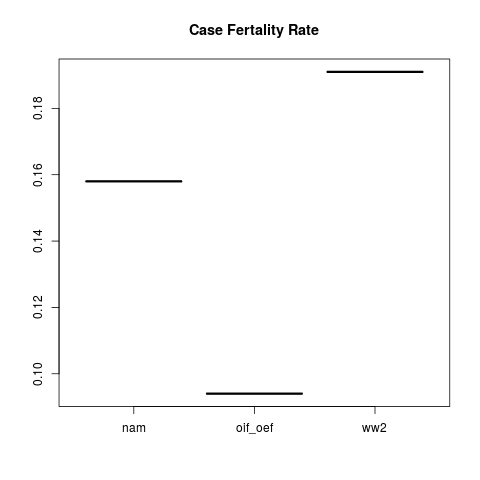
\includegraphics[width = 10cm]{cfr.png} * The
success has been proven numerically with casualty fatality rate at 19\%
during WWII, to 15.8\% during the Vietnam War, to finally 9.4\% during
Operation Iraqi Freedom (Holcomb et al J Trauma 2006) * Slow transitions
are being made to incorporate this assessment and treatment strategy
with emergency medical services, known as TECC
(http://www.naemt.org/education/tecc/what-is-tecc, Callaway UFF TC PDF)
* However, as stated previously, emergency services are delayed during
active shooter scenarios and this puts victims at risk for treatment
that is too late * Average time to exsanguination from wound hemorrhage
*** NEEDED * Airway background data*** NEEDED * We hypothesize if the
civilians in public settings are trained with similar combat casualty
care, they can learn to assess, treat, and solve the most common causes
of death during disaster scenarios and improve life expectancy.

Materials and Methods * Participants of the study were obtained as
volunteers from the city of Westminster * Laypeople include Nursing
grads and undergrads, Teachers, city workers, security guards, and
students * Teachers, city workers, security guards and students were
randomly placed into 2 groups: trained individuals and untrained
individuals * Medical trained personnel include firefighters, who are
pre-trained in disaster scenario in EMS training * Trained individuals
were given a 2-hour TCCC training overview 6 weeks prior to the
experiment * Test participants were pre-screened about their basic
knowledge of disaster scenario, with questions including ``What is the
primary cause of death in population ages 1-44?'', ``What do you think
is the standard response time when 911 is called?'', and ``What is your
primary concern immediately following a disaster or emergency
situation''. * Every group was brought individually into a room with the
chief of police, who informed them of the situation: At the mall with
friends when a magnitude 7 earthquake strikes. There will be debris on
the ground and light will be limited. You are tasked with assessing the
situation and responding. * The room was situated to simulate a major
earthquake with debris and lighting problems with 4 victims: 1 deceased,
1 arterial bleeding, 1 unconscious but breathing, and 1 healthy
individual. * The participants 1st action times and time to solution
were recorded by an observer playing a victim's friend. * Data was
recorded per each individual group and average times of trained,
untrained, and professionally trained individuals were compared to both
the arterial bleeding and airway stations

Results:

\end{document}
